\chapter{Results and Applications}

This chapter showcases numerous results generated using the estimation
technique outlined in Chapter \ref{chap:theory}. Sections \ref{sec:onedim} and
\ref{sec:twodim} focus on results generated on \ac{1D} and
\ac{2D} amplitude/phase-modulated paired datasets, respectively. The subsequent
three sections showcase three distinct applications that estimation
facilitates. In Section \ref{sec:pure-shift}, a means of generating broadband
homodecoupled (pure shift) spectra through estimation of hypercomplex \ac{2DJ}
datasets is provided. Section \ref{sec:seq} highlights how a standard \ac{1D}
estimation routine can be extended to datasets featuring a series of \acp{FID}
which feature attenuations in signal amplitudes across increments, such as
inversion recovery ($T_1$) and diffusion experiments. Finally, a protocol to
achieve ultra-broadband spectra through application of a single \ang{90}
frequency-swept pulse, which are devoid of quadratic phase dependencies as well
as severe baseline distortions, is provided. All the results and applications
presented here were acquired using the \ac{EsPy} package, which is described in
Chapter \ref{chap:nmrespy}. Relevant information on the setup of simulations
and experiments can be found in Appendix \ref{chap:datasets}. \note{Result
metics?}

\section{\acs{1D} Datasets}

In order to assess the estimation routine proposed in Chapter \ref{chap:theory}
-- specifically the effectiveness of applying \ac{NLP} using an initial guess
generated using the \ac{MPM} -- a series of synthetic \acp{FID} were constructed
using \eqref{eq:hypercomplex-fid}. For each \ac{FID}, a model order of $M=20$
was used, the number of points sampled was $\None = 1024$, the sweep width
was $\fswone=\qty{125}{\hertz}$, and the transmitter offset was $\foffone =
\qty{0}{\hertz}$.  Each oscillator was assigned a phase of \ang{0}, while the
amplitudes, frequencies and damping factors were drawn at random from the
following distributions:
$\bdam \sim \mathcal{U}(1, 5)$, $\bdfonem \sim \mathcal{U}(\qty{-55}{\hertz},
\qty{55}{\hertz})$, $\bdetaonem \sim \mathcal{U}(\qty{2}{\per\second},
\qty{8}{\per\second})\ \forall m \in \lbrace 0, \cdots, 19\rbrace$. An extra
constraint was applied to the frequencies,
such that no two oscillators were permitted to have frequencies that differed
by less than $\nicefrac{4 \fswone}{\None} \approx \qty{0.49}{\hertz}$. Each
noiseless \ac{FID} was then corrupted with \ac{AWGN}, with a target \ac{SNR} of
\qty{25}{\deci\bel}\note{Reference that this is the lowest
SNR that the MPM considered to be effective}. The spectra of the simulated
\acp{FID} are presented in panel a of Figure \ref{fig:mpm_vs_nlp}.

For each \ac{FID}, the \ac{MPM} was performed, assuming that the model order is
30, constituting a considerable over-fit. Simulated signals typically show a
clean division between signal and noise components, with noise components
commonly being characterised by small amplitudes and/or very small damping
factors. For this reason, prior to subjecting the \ac{MPM} result to \ac{NLP},
oscillators which satisfied either $\bdam < 0.1$ or  $\bdetaonem <
\qty{0.7}{\per\second}$ were removed from the parameter set. The individual
oscillators which make up the \ac{MPM} result after purging are displayed in panel b of
Figure \ref{fig:mpm_vs_nlp}, along with the residual between the data and the
model.

It can be seen that in several spectral regions across the datasets, especially
those which are more crowded, oscillators possess parameters which deviate
significantly from the true parameters (the true set of oscillators is
presented in panel d), with the most notable feature being individual
oscillator phases, which can stray far from \ang{0}.
The central motivation behind employing phase variance-regularised \ac{NLP} is
as a means of attempting to overcome this detrimental feature of the \ac{MPM}.
It should be noted however, that the \ac{MPM} invariably generates a model with
good agreement with the data, as evidenced by the residual.
In Figure \ref{fig:mpm_vs_nlp}, the blue oscillators are those which agree very
closely with a particular oscillator in the true set of parameters. Oscillators
with other colours are in disagreement for some reason (\textit{vide infra}).
The goal of the \ac{NLP} routine is therefore to adjust the parameters
describing the non-blue oscillators in panel b such that they agree with
oscillators found in the true set, while not affecting the blue oscillators.
The results of \ac{NLP} at convergence ($\epsilon = \num{1e-8}$) are provided
in panel c. ...

\note{Maybe define the notion of a ``frequency neighbourhood''?
    A small rage of frequencies within which it is necessary for the MPM to generate at least the same number of oscillators as the true number for NLP to have a chance of correctly estimating the dataset.
}

\paragraph{Green oscillators}
These oscillators belong to a grouping of oscillators with similar frequencies
which exhibited significant deviation from the true parameter set, but which
were mapped to agree closely with the true result thanks to the \ac{NLP}
routine.

\paragraph{Orange oscillators}
Orange oscillators are examples of scenarios where the \ac{MPM} routine
over-fit a particular spectral region, and the \ac{NLP} routine was able to
purge these excessive oscillators, leading to a parsimonious set of parameters.

\paragraph{Red oscillators}
These oscillators are examples of a cases where the routine has underfit the
dataset, because there are a pair of similar-frequency oscillators in the true
parameter set which were not be individually resolved. In these cases, the
\ac{MPM} assigned only a single oscillator to fit the spectral region, making
it impossible for the \ac{NLP} routine to make any improvements to the
estimation result.

\paragraph{Yellow oscillators}
Similar to red oscillators, yellow oscillators eventually lead to the
under-fitting of the dataset. However, in these cases, the \ac{MPM} has
generated sufficient oscillators in the frequency neighbourhood. Unlike in
scenarios which is seen for the green oscillators though, the \ac{NLP} routine
evolves such that at least one of the oscillators is driven by the phase
variance constraint to acquire a negative amplitude, such that it is purged
from the parameter set. This typically occurs when an oscillator has an initial
phase close to \ang{180}.

\paragraph{Purple oscillators}
The arise rather infrequently, and correspond to over-fits of the dataset.


\begin{sidewaysfigure}
    \centering
    \includegraphics{mpm_vs_nlp/mpm_vs_nlp.pdf}
    \caption[
        The result of estimating a series of 5 simulated signals comprising 20
        oscillators, using solely the \acs{MPM} and also with phase
        variance-regularised \acs{NLP} afterwards.
    ]{
        The result of estimating a series of 5 simulated signals comprising 20
        oscillators (see the main text for details on how the datasets were constructed).
        \textbf{a.} Spectra of the datasets generated.
        \textbf{b.} Plots of spectral lines for each oscillator generated using
        the \acs{MPM}.
        \textbf{c.} An equivalent plot for the result after applying \acs{NLP},
        with the \ac{MPM} result being the initial guess.
        \textbf{d.} Spectral lines corresponding to the true set of oscillators
        used to generate each the datasets.
        Also included in \textbf{b.} -- \textbf{d.} is the residual between the
        data and the sum of the oscillator peaks (grey line).
        The colouring of oscillator lines is described in the main text.
    }
    \label{fig:mpm_vs_nlp}
\end{sidewaysfigure}

\section{\acs{2D} Datasets}
\label{sec:twodim}

\section{Pure-Shift Spectra via \acl{2DJ} Estimation}
\label{sec:pure-shift}

Two key features which the \ac{NMR} community is constantly seeking to improve
are the sensitivity and resolving power of experiments. There are
numerous means of improving spectral sensitivity, via technological
advancements including the production of superconducting magnets with higher
field strengths\note{CITE?} (sensitivity $\propto B_0^{\nicefrac{7}{4}}$),
and cryogenic probes\cite{Kovacs2005}, as well as simply increasing the number
of scans (\ac{SNR} $\propto \text{NS}^{\nicefrac{1}{2}}$).  There are however
few means of achieving better resolution beyond increased field strengths
(resolution $\propto B_0$). Significant interest has therefore been
given to the development of homodecoupled (``pure shift'')
experiments\cite{Meyer2013,Adams2014,Zangger2015}, in which the
effects of homonuclear scalar couplings are removed from the data. The presence
of J-couplings, indicating the close proximity of spins in a chemical
bonding sense, is a distinguishing feature of \ac{NMR}, and is often valuable for
structural assignment. However, in many cases their effect can lead to spectra
which are too crowded for meaningful insights to be gleamed.  Heteronuclear
couplings, between spins with different nuclei (i.e. \proton\ and \carbon) are
straightforward to decouple at the point of \ac{FID} acquisition, using well
known schemes such as WALTZ-16\cite{Shaka1983a, Shaka1983b} and
GARP\cite{Shaka1985}. Homonuclear decoupling is anything but simple on the
other hand.

In this section, an overview of the key techniques which have
been developed to generate pure shift spectra is given, starting with \ac{2DJ}
spectroscopy and finishing up with \ac{PSYCHE}, widely considered the most
robust pure shift experiment in terms of sensitivity and tolerance to strong
coupling. Subsequently, a new technique for generating pure shift spectra via
parametric estimation, named \acf{CUPID} is presented.

\subsection{An Overview of Pure Shift NMR}

\subsubsection{The \acl{2DJ} Experiment}
The \ac{2DJ} experiment\cite{Aue1976, Morris2009} provided the first means of
achieving pure shift spectra.  It has a simple pulse sequence, presented in
Figure \ref{fig:pure_shift_seqs}.a: after excitation of magnetisation onto the
transverse plane, the indirect dimension evolution consists of a spin echo, with
acquisition following immediately afterwards. Fourier transformation in both
dimensions leads to a spectrum in which only scalar couplings contribute in
$\Fone$, as the chemical shifts are refocussed by the spin echo, while both
scalar couplings and chemical shifts contribute in $\Ftwo$.
Peaks belonging to a particular multiplet lie along a line at \ang{45} to the
$F^{(1)}$ and $F^{(2)}$ axes, as seen in panel a. of Figure
\ref{fig:jres_spectrum}.
\begin{figure}%
    \centering%
    \includegraphics{jres_spectrum/jres_spectrum.pdf}%
    \caption[
        Example of a simple \acs{2DJ} spectrum derived from an AMX spin system.
    ]
    {%
        \textbf{a.} Contour plot of an absolute value mode \ac{2DJ} spectrum for an
        AMX spin system, produced by applying sine-bell apodisation on a hypercomplex
        \ac{FID} before a \ac{FT} in both dimensions. Each multiplet lies a
        long a line at \ang{45} to the $F^{(1)}$ and $F^{(2)}$ axes. Note that
        this line often appears to make an angle that is greater than \ang{45}
        with the $F^{(2)}$ axis when viewing spectra, since typically $\fswone
        \ll \fswtwo$. Above the \ac{2DJ} spectrum is a plot of its summation
        along the $\Fone$ axis.
        \textbf{b.} Spectrum generated after application of a \ang{45} shear,
        with its $\Fone$ summation above.
   }%
    \label{fig:jres_spectrum}%
\end{figure}%

An FID generated by the \ac{2DJ} experiment is hypercomplex, taking the form of
\eqref{eq:general fid} with $D=2$ and $\zeta = \exp(\iu\cdot)$, i.e.
\begin{equation}%
    \begin{split}%
        \jresfid\idxnonentwo =
        \sum_{m=0}^{M-1} \bdam \exp\left( \iu \bdphim \right)
            \exp\left(\left(2 \pi \iu \bdfonem - \bdetaonem\right) {\none}_{\vphantom{t}} \Dtone\right) \times \\
            \exp\left(\left(2 \pi \iu \bdftwom - \bdetatwom\right) {\ntwo}_{\vphantom{t}} \Dttwo\right)
            + \symbf{W}\left[n^{(1)}, n^{(2)}\right].
    \end{split}%
    \label{eq:jres-fid}
\end{equation}%
A major downside of the \ac{2DJ} experiment is there is no means of generating
a pair of phase- or amplitude-modulated signals which are the
conventional route to frequency-discriminated spectra with absorption mode
lineshapes. In many multidimensional experiments, changing the phase of
certain \ac{RF} pulses or the use of \acp{PFG} can induce a change in the \ac{CTP},
generating such signal-pairs, though this unavailable with \ac{2DJ}
spectroscopy as no mixing time exists. The FT of $\jresfid$ produces a spectrum
$\jresspec$ with ``phase-twist'' peaks, which possess contributions from both absorption
and dispersion Lorentzians. There are two primary steps involved in obtaining a
pure shift spectrum from $\jresspec$:
\begin{enumerate}
    \item Perform a \ang{45} shear (often called a tilt) on the spectrum array,
        leading to the separation of chemical shifts and scalar couplings onto
        orthogonal axes  (panel b. in Figure \ref{fig:jres_spectrum}). Each
        slice in $\Ftwo$ is subjected to a right circular rotation such that
        \begin{subequations}
            \begin{gather}
                \jresspectilt\left[{\none}\vpsub{\mathrm{sw}},{\ntwo}\vpsub{\mathrm{sw}}\right] =
                \jresspec\left[{\none}\vpsub{\mathrm{sw}},\ntwonew\right],\\
                \ntwonew = \left(
                    {\ntwo}\vpsub{\mathrm{new}} + \left\lfloor
                        \frac
                            {\fswone \Ntwo\vpsub{\mathrm{sw}}}
                            {\fswtwo \None\vpsub{\mathrm{sw}}}
                        \left(
                            \frac{\None\vpsub{\mathrm{sw}}}{2} - \none
                        \right)
                    \right\rceil
                \right) \bmod \Ntwo.
            \end{gather}
        \end{subequations}
        This achieves the mapping $\jresspec\left(\fone,\ftwo\right)
        \rightarrow \jresspec\left(\fone, \ftwo - \fone\right)$.  It should be
        noted that the effectiveness of the shear is maximised when both
        $\nicefrac{\fswtwo}{\fswone}$ and $\nicefrac{\Ntwo}{\None}$ are powers
        of 2\note{check this}.
    \item Sum the spectrum along $\Fone$:
        \begin{equation}
            \specps\idxntwo =
            \sum_{\none=0}^{\None-1} \jresspectilt\idxnonentwo.
        \end{equation}
\end{enumerate}%
Shearing and summing $\jresspec$ actually leads to the absorptive and dispersive
components of the spectrum cancelling each other out . It is necessary to display
the spectrum in absolute value mode before carrying out the above steps (i.e.
use $\Re(\lvert \jresspec \rvert)$).
This still leads to undesirable pure shift spectra with broad ``wings'' on
account of the presence of dispersive character. The dispersive component can
be suppressed by appropriate processing to make the FID envelope symmetric in
both dimensions, such as with sine-bell
apodisation\cite[Section3.3.5]{Lindon1980}, or pseudo-echo
reshaping\cite{Bax1981}, though this results in a significant reduction in
sensitivity being incurred.

\begin{figure}
    \centering
    \includegraphics{pure_shift_sequences/pure_shift_sequences.pdf}
    \caption[
        The pulse sequences of some common pure shift experiments.
    ]{
        \note{Work needed. Figure out the correct delays in ZS, BIRD, PSYCHE}
        The pulse sequences of four of the most common pure shift experiments.
        \textbf{a.} \acs{2DJ}.
        \textbf{b.} The \acs{ZS} method.
        \textbf{c.} The \acs{BIRD} method.
        \textbf{d.} The \acs{PSYCHE} method.
    }
    \label{fig:pure_shift_seqs}
\end{figure}

\subsubsection{The \acl{ZS} Method}
\label{subsec:ZS}
In 1997 Zangger and Sterk introduced a pulse sequence element which achieves
slice-selective excitation, by applying a low \ac{RF} power (weak) \ang{180}
pulse\footnote{Conventionally, a R-SNOB pulse is used\cite{Kupce1995}.} in the
presence of a \ac{PFG} along the $z$-axis\cite{Zangger1997}. Such an element
excites a
given spin only in a narrow range of heights in the sample, as the \ac{PFG}
induces a shift in resonance frequency according to $\Delta \omega(z) = \gamma
G_z z$, where $G_z$ is the magnitude of the \ac{PFG}. By placing a hard
\ang{180} pulse adjacent to the selective pulse, the
``active'' spin in a given slice is rotated by \ang{360} (i.e. no net
rotation), while all other (``passive'') spins are only rotated by \ang{180}.
Placing such a element in the middle of the $\tone$ evolution therefore
achieves refocussing of the J-couplings associated with the active
spin\cite{Aguilar2010}. In order to achieve effective decoupling of any given
pair of spins, it is necessary that the bandwidth of the selective π-pulse is
smaller than the difference in their chemical shifts. However, with more
selective pulses, a smaller proportion of the available spin magnetisation will
contribute to the final FID, and hence sensitivity will be diminished
\footnote{
    The reduction in sensitivity is $\propto \nicefrac{f_B}{\gamma G_z l_z}$,
    where $f_B$ is the selective pulse bandwidth, and $l_z$ is the length of
    the sample lying within the receiver coil ($\approx
    \qty{1.5}{\centi\meter}$).
}.
There is therefore a trade-off between effective decoupling of all spins, and
achieving the greatest sensitivity possible. In the case of strong coupling,
the \ac{ZS} method tends to perform poorly relative to other options for this
reason. The \ac{ZS} element has been applied by Keeler and Pell in order to
generate \ac{2DJ} datasets comprising phase-modulated pairs, enabling the
generation of pure absorption-mode spectra\cite{Pell2007}.


\subsubsection{The \acs{BIRD} Method}
The \ac{BIRD} pulse sequence element\cite{Garbow1982,Bax1983}, presented in
Figure \ref{fig:pure_shift_seqs}.c, also takes advantage of the idea of
selectively inverting passive spins, while leaving active spins unaffected.
However the active spins are those which are directly bound to
\textsuperscript{13}C nuclei, which naturally occur with an abundance of 1.1\%,
while the passive spins are those bound to far more abundant
\textsuperscript{12}C nuclei. The reduction in sensitivity of the experiment
relative to a full-sensitivity experiment is therefore known and constant
across samples. In scenarios where is this strong coupling, \ac{BIRD} can
achieve improved sensitivity over \ac{ZS}, since with the latter a very weak
selective pulse would be required to ensure it is of a sufficiently small
bandwidth. The \ac{BIRD} method is particularly attractive in scenarios where
the sensitivity penalty due to the involvement of a low-abundance nucleus has
already been paid, for example in a \ac{HSQC} experiment\cite{Paudel2013}.

\subsubsection{PSYCHE}
\label{subsec:psyche}
\note{TODO}
Original paper\cite{Foroozandeh2014}, tutorial paper\cite{Foroozandeh2018}, PSYCHE-2DJ\cite{Kiraly2017}.

\subsubsection{Pure Shift NMR via J-Resolved Post-Processing}

There have been previous descriptions of acquiring pure-shift spectra from
typical \ac{2DJ} datasets via more sophisticated post-processing methods.
Nuzillard presented \ac{ALPESTRE}\cite{Nuzillard1996}, in which the parameters
of each indirect-dimension FID are estimated using linear prediction, such that
there is a set of parameters $\symbf{\Theta} \in \mathbb{R}^{\Ntwo \times 4M}$
with
\begin{equation}
    \symbf{\Theta}\left[\ntwo\right] =
    \begin{bmatrix}
        \left[\bda_{\ntwo}\right]\T &
        \left[\bdphi_{\ntwo}\right]\T &
        \left[\bdfone_{\ntwo}\right]\T &
        \left[\bdetaone_{\ntwo}\right]\T
    \end{bmatrix}.
\end{equation}
The parameters generated are used to propagate each FID backward into
$-\tone$, producing a ``full-echo'':
\begin{equation}
    \begin{split}
        \symbf{Y}_{\text{full}}\left[\none, \ntwo\right] = \sum_{m=0}^{M-1}
            \bda_{\ntwo} \left[ m \right]
            \exp\left(\iu \bdphi_{\ntwo} \left[ m \right] \right)
            \exp\left(\left(2 \pi \iu \bdfone_{\ntwo} \left[ m \right] \none
            -\bdetaone_{\ntwo} \left[ m \right] \left\lvert \none \right\rvert \right)\Dtone\right) \\
        \forall \none \in \mathbb{Z}: -\None < \none < \None,\\ \forall \ntwo \in \mathbb{N}_0: \ntwo < \Ntwo.
    \end{split}
\end{equation}
\ac{FT} of generates a spectrum whose real component comprises absorption-mode
Lorentzian character in both dimensions. This opens up the means of producing
pure-shift spectra from the \ac{2DJ} experiment with sharp lineshapes and
without sensitivity loss. A similar approach proposed by Mutzenhardt et al.
instead constructed full echoes via \ac{LP} of each direct-dimension
\ac{FID}, and generation of a full echo by propagating
into $-\ttwo$\cite{Mutzenhardt1999}.

\subsection{An outline of \acs{CUPID}}
\ac{CUPID} aims to generate pure shift spectra by utilising the result of
parametric estimation on \ac{2DJ} data, assumed to take the functional form of
\eqref{eq:jres-fid}.
Instead of estimating successive \ac{1D} \acp{FID}, as has been described by
Nuzillard and Mutzenhardt et al., the entire \ac{2DJ} signal is estimated as a
whole, giving access to the parameter vector $\bth \in \mathbb{R}^{6M}$. Using
$\bth$, a synthetic \ac{1D} \ac{FID}, named the ``\ang{-45} signal'' (Figure
\ref{fig:neg-45}), is produced:
\begin{equation}
    \symbf{y}_{\ang{-45}}\left(\bth\right)\left[ \ntwo \right] =
        \sum_{m=0}^{M-1} \bdam \exp \left(\iu \bdphim \right)
        \exp\left(
            \left(
                2 \pi \iu \left(\bdftwom - \bdfonem\right)
                - \bdetatwom
            \right) \ntwo \Dttwo
        \right).
    \label{eq:neg-45}
\end{equation}
$\forall \ntwo \in \lbrace 0, \cdots, \Ntwo - 1 \rbrace$. The \ang{-45} signal
takes the same functional form as a typical \ac{1D}
\ac{FID} acquired by a pulse-acquire experiment, except that the frequency of
each oscillator, which would usually be $\ftwo$, is replaced with $\ftwo -
\fone$. In a \ac{2DJ} experiment, $\fone$ corresponds to the displacement of a
given oscillator from the central frequency of the multiplet it is associated
with. As such, the oscillators belonging to a given multiplet all provide
a contribution with the same frequency to the \ang{-45} signal, namely the
chemical shift of relevant spin.
\begin{figure}
    \centering
    \includegraphics{neg_45_signal/neg_45_signal.pdf}
    \caption[
        An illustration of the reasoning behind the name ``\ang{-45}
        signal''.
    ]{
        An illustration of the reasoning behind the name ``\ang{-45}
        signal''. The pale red dots denote a typical \ac{2DJ} \ac{FID}, where
        the amount and rate of sampling in the direct dimension is greater than
        in the indirect dimension (i.e. $\None \ll \Ntwo$ and $\fswone \ll
        \fswtwo$). The bright red dots correspond to the first direct-dimension
        signal $\bY_{\text{2DJ}}(0, \ttwo)$, which has the same form as
        \iac{FID} from a pulse-acquire experiment. A hypothetical signal
        generated by propagating the \ac{FID} into $-\tone$, with the same rate
        of sampling in both dimensions, is denoted with pale blue dots. Taking
        the diagonal of this signal, such that it forms a \ang{-45} to the
        $\ttwo$ axis, yields an \ac{FID} $\by_{\ang{-45}}$  which is
        homodecoupled. It should be noted that there is a slightly discrepancy
        between \eqref{eq:neg-45} and this description, in that the
        indirect-dimension damping factors $\bdetaone$ are neglected in the
        former case.
    }
    \label{fig:neg-45}
\end{figure}

\subsubsection{Multiplet Prediction}
A holistic \ac{2D} estimation of the \ac{FID} provides access to other useful
information about the dataset. One such example is the grouping of oscillators
in account of which multiplet structure they belong to. As has already been
established, for oscillators which are associated with the same multiplet
structure, the quantity $\ftwo - \fone$ should be equal. This provides a
criterion in order to assess whether it is likely that two oscillators in the
estimation result belong to the same multiplet:
\begin{equation}
    \left \lvert
        \left( \bdftwo \left[ m_1 \right] -
        \bdfone \left[ m_1 \right] \right) -
        \left( \bdftwo \left[ m_2 \right] -
        \bdfone \left[ m_2 \right] \right)
    \right \rvert < \epsilon
\end{equation}
$\forall m_1, m_2 \in \lbrace 0, \cdots, M-1 \rbrace$, with  $\epsilon \in
\mathbb{R}_{>0}$ being a suitable threshold to account for error in the
estimation. An appropriate value for $\epsilon$ would appear to be half the
spectral resolution in the more poorly resolved dimension, i.e.
$\epsilon = \min\left(\nicefrac{\fswone}{2 \None}, \nicefrac{\fswtwo}{2\Ntwo}\right)$. In situations involving real \ac{2DJ}
signals however, it is found that $\epsilon$ sometimes has to be increased to
values slightly larger than this to achieve effective groupings (\textit{vide
infra}). Algorithm \ref{alg:mp-assign} provides a routine that can be used for
multiplet prediction.

\note{Removal of spurious oscillators}

\subsubsection{Filtration of \ac{2DJ} data}
Unlike the direct-dimension, which can often comprise sparsely distributed
peaks in the Fourier domain, the indirect dimension of \ac{2DJ} datasets tends
to be rather densely populated. As such, it is typically of little use in
attempting to generate filtered sub-\acp{FID} in the indirect dimension. The
filtering procedure utilised for \ac{2DJ} data is therefore an extension of the
filtration procedure for \ac{1D} data described in Section \ref{sec:filtering}
(Figure \ref{fig:jres-filtering}). The filtering procedure involves the
following steps:
\begin{enumerate}
    \item The signal $\symbf{Y}_{\text{ve}} \in \mathbb{C}^{\None \times 2 \Ntwo}$ is
    constructed, such that a virtual echo is formed from each direct-dimension
    signal:
    \begin{equation}
        \begin{split}
            \symbf{Y}_{\text{ve}} \left[n^{(1)}\right] =
                &\left[
                \begin{matrix}
                    \Re\left(\symbf{Y}\left[n^{(1)}, 0\right]\right) &
                    \symbf{Y}\left[n^{(1)}, 1\right] &
                    \cdots
                \end{matrix}\right.
                \\
                &\left.
                \begin{matrix}
                    \symbf{Y}\left[n^{(1)}, \Ntwo - 1\right] &
                    0 &
                    \symbf{Y}\left[n^{(1)}, \Ntwo - 1\right]^* &
                    \cdots &
                    \symbf{Y}\left[n^{(1)}, 1\right]^*
                \end{matrix}
                \right]
        \end{split}
    \end{equation}
    $\forall n^{(1)} \in \lbrace 0, \cdots, N^{(1)} - 1 \rbrace$.
    \item $\symbf{Y}_{\text{ve}}$ is subjected to \ac{FT} along the direct
        dimension to produce the spectrum  $\symbf{S}_{\text{ve}}$ (panel a of
        Figure \ref{fig:jres-filtering}). This has a imaginary component of
        zeros.
    \item A super-Gaussian $\symbf{G} \in \mathbb{R}^{\None \times 2 \Ntwo}$ is
        constructed (panel b):
        \begin{equation}
            \symbf{G} = \symbf{1} \otimes \symbf{g}^{(2)},
        \end{equation}
        where $\symbf{1} \in \mathbb{R}^{\None}$ is a vector of ones, and
        $\symbf{g}^{(2)}$ is a super-Gaussian vector given by
        \eqref{eq:super-Gaussian-onedim} with $d=2$.
    \item A matrix of additive noise is generated by extracting the variance
        $\sigma^2$ of a strip of $\symbf{S}_{\text{ve}}$ which is devoid of
        peaks, and generating an array $\symbf{W}_{\sigma^2} \in
        \mathbb{R}^{\None \times 2 \Ntwo}$ with values independently sampled
        from a normal distribution with mean $0$ and variance  $\sigma^2$.
    \item The spectrum is filtered according to \eqref{eq:Sve-tilde}, yielding
        $\widetilde{\symbf{S}}_{\text{ve}}$ (panel d).
    \item $\widetilde{\symbf{S}}_{\text{ve}}$ is subjected to \ac{IFT} and is
        slicing in half in the direct dimension, yeilding the final filtered
        signal $\widetilde{\symbf{Y}}$:
        \begin{equation}
            \widetilde{\symbf{Y}} = \IFT^{(2)}\left(\widetilde{\symbf{S}}_{\text{ve}}\right) \left[:, : \Ntwo\right].
        \end{equation}
\end{enumerate}

\begin{figure}
    \centering
    \includegraphics{jres_filtering/jres_filtering.pdf}
    \caption[
        An illustration of the filtering procedure for \ac{2DJ} data.
    ]
    {
        An illustration of the filtering procedure for \ac{2DJ} data.
        For each panel is a heat-map of the full \ac{2D} signal, as well as a
        plot underneath of the first slice of the signal in the direct
        dimension.
        \textbf{a.} The spectrum $\symbf{S}_{\text{ve}}$,
        \textbf{b.} Super-Gaussian filter $\symbf{G}$,
        \textbf{c.} Additive noise, attenuated by the super-Gaussian, $\symbf{W}_{\sigma^2} \odot (\symbf{1} - \symbf{G})$,
        \textbf{d.} Filtered spectrum $\widetilde{\symbf{S}}_{\text{ve}}$
        Panels \textbf{a.}--\textbf{d.} are analogous to panels \textbf{b.}--
        \textbf{e.} in Figure \ref{fig:filtering} for the \ac{1D} case.
    }
    \label{fig:jres-filtering}
\end{figure}

\subsection{Results Using \acs{CUPID}}
\label{subsec:cupid-results}
A number of examples of the application of \ac{CUPID} are now provided.
Initially, a few results are presented using data simulated using the Spinach
MATLAB\textregistered\ library\cite{Hogben2011}.
After this, examples are provided with experimental data. In a couple of these,
comparison of the result acquired using \ac{CUPID} is compared with a spectrum
acquired using \ac{PSYCHE}.

For additional details relating to generation of the simulated datasets, see
section \ref{sec:simulated-datasets} in the Appendix.

\subsubsection{``Four Multiplets''}
\begin{figure}
    \centering
    \includegraphics{four_multiplets/four_multiplets}
    \caption[
        The result of applying \acs{CUPID} to 5 instances of simulated
        \acs{2DJ} datasets with 4 heavily overlapping multiplet structures.
    ]{
        The result of applying \ac{CUPID} to 5 instances of simulated \ac{2DJ}
        datasets with 4 heavily overlapping multiplet structures.
        \textbf{a.} Black: pure shift spectrum generated by \ac{CUPID}.
        Grey: \ac{1D} spectrum simulated with Spinach, using the same spin
        system as was used to produce the \ac{2DJ} dataset, but with all scalar
        couplings sets to \qty{0}{\hertz}. This has been offset slightly for
        clarity.
        \textbf{b.} \ac{1D} spectrum of the dataset.
        \textbf{c.} Multiplet structures predicted, using a threshold $\epsilon
        = \nicefrac{\fswtwo}{2 \Ntwo} \approx \qty{0.49}{\hertz}$.
        \textbf{d.} Contour plot of the \ac{2DJ} spectrum in absolute-value
        mode. Coloured points denote the frequencies of oscillators in the
        estimation result.
        Coloured vertical lines denote the predicted central frequencies of
        each multiplet structure.
    }
    \label{fig:four-multiplets}
\end{figure}
A series of simulated \proton\ \ac{2DJ} datasets were generated such that
within a known region of the spectrum, four ddd multiplet structures with
significant overlap existed. To achieve this, a spin-system with 7 spins was
formed, with the spins divided into 2 subsets:
\begin{itemize}
    \item 4 of the spins (the ``estimated spins'') were assigned random
        resonance frequencies sampled from $\mathcal{U}(\qty{-20}{\hertz},
        \qty{20}{\hertz})$.
    \item The remaining 3 spins (the ``coupling spins''), were coupled to each
        of the estimated spins, with the values of the couplings randomly
        sampled from $\mathcal{U}(\qty{-10}{\hertz}, \qty{10}{\hertz})$.  The
        coupling spins were given chemical shifts such that they lay far from
        the estimated spins in the spectrum (i.e. their frequencies were $\gg
        \qty{20}{\hertz}$).
\end{itemize}
\ac{AWGN} noise was added to the \ac{FID}, with a target \ac{SNR} of \qty{30}{\deci\bel}.
A filtered sub-\ac{FID} containing only the signals from the estimated spins
was then generated using the filtering procedure described above, with
$l^{(2)}_{\unit{\hertz}} = \qty{30}{\hertz}$,
$r^{(2)}_{\unit{\hertz}} = \qty{-30}{\hertz}$, and
$\xi = 1.1$. The resulting sub-\ac{FID} was expected to comprise 32 ($4 \times
2^3$) oscillators. To assess the estimation procedure's ability, a random
integer from the range 33 -- 40 was selected as the initial number of
oscillators. Hence, the initial guess from the \ac{MMEMPM} would comprise an
excessive number of oscillators. The \ac{FID} was subjected to
estimation, yielding the result vector $\bthstar$. Spurious oscillators were
checked for, using the criteria outlined above, with the threshold for
multiplet assignment set to half the spectral resolution in the direct
dimension:
$\epsilon = \nicefrac{f_{\text{sw}}^{(2)}}{2\Ntwo}$.  If spurious oscillators
were found, these were removed, and \ac{NLP} was run on the updated set of
parameters.

Figure \ref{fig:four-multiplets} illustrates the result achieved for 5 separate
runs of the procedure described above.
For each \ac{FID} generated, the method was effective at producing an
estimation result with 32 oscillators, as desired, despite the excessive number
that were present in $\bthzero$. Most of the excessive oscillators were purged
from $\bthzero$ through the \ac{NLP} procedure. When spurious oscillators did
remain\footnote{for 2 of the 5 datasets, the result after \ac{NLP} comprised 33
oscillators}, they were then detected when checking for spurious oscillators
and subsequently removed. The pure-shift spectra generated using \ac{CUPID}
closely agree with pure-shift spectra generated by running a Spinach simulation
on a spin system with the same chemical shifts, but with all scalar couplings
set to \qty{0}{\hertz}.

\subsubsection{``Sucrose''}
\begin{figure}
    \centering
    \includegraphics{sucrose_cupid/sucrose_cupid.pdf}
    \caption[
        Application of \acs{CUPID} on a simulated sucrose \acs{2DJ} dataset.
    ]
    {
        Application of \ac{CUPID} on a simulated sucrose \ac{2DJ} dataset.
        \textbf{a.} Black: the spectrum generated from \ac{FT} of the \ang{-45}
        signal. Grey: the spectrum of a simulated dataset with the same
        chemical shifts, with all scalar couplings set to \qty{0}{\hertz}.
        \textbf{b.} Conventional \ac{1D} spectrum.
        \textbf{c.} Multiplet structures assigned ($\epsilon \approx
        \qty{0.27}{\hertz}$).
        \textbf{d.} Contour plot of the absolute value mode \ac{2DJ} spectrum,
        with the locations of assigned oscillators given as coloured points.
    }
    \label{fig:sucrose-cupid}
\end{figure}
As a second example of applying \ac{CUPID} on simulated data, the chemical
shifts and isotropic scalar couplings associated with a
Gaussian\cite{Gaussian03} \ac{DFT} calculation of sucrose in a vacuum
\footnote{
It is well known that isotropic chemical shift calculations using \ac{DFT} are
typically very inaccurate. The resulting spectrum is not typical of sucrose in
the liquid state, though this doesn't really matter for assessing the
performance of \ac{CUPID}.
}
were used to construct a 2DJ dataset. \ac{AWGN} was added with a target
\ac{SNR} of \qty{20}{\deci\bel}. The CUPID procedure was applied to filtered
sub-FIDs such that the resonances from all 22 spins were considered, though
only the regions of the dataset with the most interesting multiplet structures
are presented in Figure \ref{fig:sucrose-cupid}.

The estimation technique successfully assigned multiplet structures for all 22
multiplets in the dataset, including structures derived from two spins (F \& N)
with a \qty{0.6}{\hertz} difference in resonance frequency, approaching the
spectral resolution in the direct dimension (\qty{0.537}{\hertz}). The
pure-shift spectrum generated via the \ang{-45} signal again showed close
agreement with a 1D spectrum simulated using the same chemical shifts, with
scalar couplings set to \qty{0}{\hertz}. There are particular multiplets where
the number of oscillators fit using the estimation routine was less than the
true number. Examples of this phenomenon are exhibited in the estimates of the
multiplets for spins B \& O, which are both ddd structures. The scalar
couplings involved meant that certain oscillators were
of such similar frequencies that they were separated by significantly less than
the spectral resolution, and thus deconvolving these was unrealistic. For
example, there are two pairs of peaks in the spin-B multiplet which lie only
\qty{0.085}{\hertz} apart. Under-fitting in this case had a negligible impact
on the final pure shift spectrum. However there are circumstances which will be
seen in the experimental examples below where more blatant cases under-fitting
lead to the generation of peaks in the pure shift spectrum which are noticeably
broadened (\textit{vide infra}).

\subsubsection{Quinine}
\begin{figure}
    \centering
    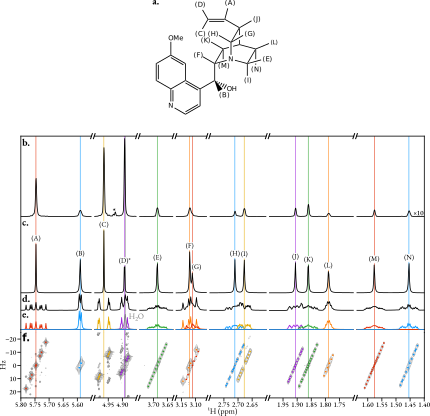
\includegraphics{quinine_cupid/quinine_cupid.pdf}
    \caption[
        Application of \acs{CUPID} on the non-aromatic regions of a quinine
        \acs{2DJ} dataset.
    ]{
        Application of \ac{CUPID} on the non-aromatic regions of a quinine
        \ac{2DJ} dataset.
        \textbf{a.} The spectrum generated from \ac{FT} of the \ang{-45}
        signal, with the green signal arising from water at about
        \qty{4.89}{\partspermillion} neglected.
        \textbf{b.} Conventional \ac{1D} spectrum.
        \textbf{c.} Multiplet structures assigned ($\epsilon =
        \nicefrac{\fswtwo}{\Ntwo} \approx \qty{0.92}{\hertz}$).
        \textbf{d.} Contour plot of the absolute value mode \ac{2DJ} spectrum,
        with the locations of assigned oscillators given as coloured points.
    }
    \label{fig:quinine-cupid}
\end{figure}

Figure \ref{fig:quinine-cupid} illustrates the result of applying \ac{CUPID} on
a dataset generated from a sample comprising quinine in CD\textsubscript{3}OD,
with all non-aromatic protons considered. The method successfully generated a
pure shift spectrum with distinct peaks for each \textsuperscript{1}H
environment. This example also highlights an added benefit of using \ac{CUPID}:
the ability to suppress unwanted signals in the final spectrum. In this
example, an intense, broad singlet at around \qty{4.89}{\partspermillion}
was detected (see the green peak at this frequency in panel c).
The singlet was due to the presence of water in the sample and was a hindrance
due to it overlapping heavily with the multiplet structure corresponding to
spin D. To obtain a clean singlet for spin D in the pure shift spectrum, the
oscillator corresponding to the water signal was simply neglected from
$\bthstar$ in generating the \ang{-45} signal. \note{Find reference for work
talking about using estimation for solvent suppression.}

As eluded to already, a few of the peaks in the pure-shift spectrum are rather
broad on account of the estimation routine under-fitting the relevant multiplet
structure. The most notable example of this phenomenon in the quinine example
comes from the peak for spin G, where siginifcant overlap with spin F has likely
compunded the task of accurately estimating the \ac{FID}. With fewer than the
true number of oscillators fitting a given multiplet structure, the \ac{NLP}
routine will compensate by giving the oscillators it does have at its disposal
large amplitudes and damping factors, so that they can reasonably fit multiple
similar-frequency oscillators.
While affecting peak linewdiths, this feature does not tend to significantly
affect the integrals of the pure shift peaks. \note{Should probably calculate
the integrals of these...}

\subsubsection{Dexamethasone}

\begin{sidewaysfigure}%
    \centering%
    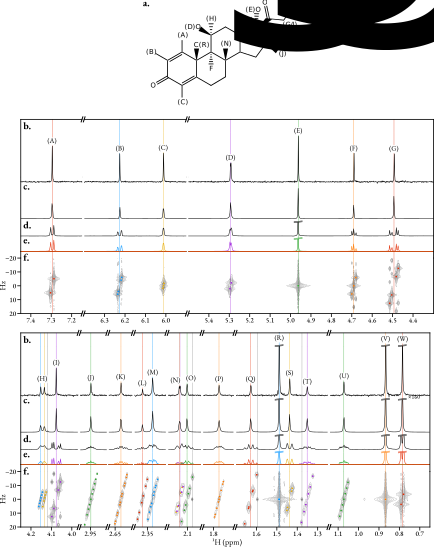
\includegraphics{dexamethasone_cupid/dexamethasone_cupid.pdf}%
    \caption[
        Application of \ac{CUPID} on a dexamethasone dataset.
    ]{
        Application of \ac{CUPID} on dexamethasone \ac{2DJ} dataset.
        \textbf{a.} \ac{TSE-PSYCHE} spectrum of the sample.
        \textbf{b.} The spectrum generated from \ac{FT} of the \ang{-45}
        signal.
        \textbf{c.} Conventional \ac{1D} spectrum.
        \textbf{.} Multiplet structures assigned ($\epsilon =
        \nicefrac{\fswtwo}{\Ntwo} \approx \qty{0.92}{\hertz}$).
        \textbf{d.} Contour plot of the absolute value mode \ac{2DJ} spectrum,
        with the locations of assigned oscillators given as coloured points.
    }
    \label{fig:dexamethasone-cupid}%
\end{sidewaysfigure}%
\note{Double check mp thold}

Figure \ref{fig:dexamethasone-cupid} shows the result of applying CUPID on a
dataset acquired from a sample dexamethasone in DMSO-d\textsubscript{6}. A
pure-shift spectrum was also acquired using the
\ac{TSE-PSYCHE} experiment\cite{Foroozandeh2018,Foroozandeh2015} for
comparison.
\ac{CUPID} generated a pure-shift spectrum with overall excellent agreement
with the PSYCHE spectrum. Certain multiplet structures in the spectrum exhibit
splitting in $\Ftwo$, on account of heteronuclear couplings to \textsuperscript{19}F. Most
notable are those derived from spins D, H \& O. For the D multiplet, the
magnitude of $J_{\textsuperscript{1}H,\textsuperscript{19}F}$ is very small
such that assigning these to separate oscillators is infeasible.
For the spin N multiplet, two separate structures were successfully assigned
(see the orange and green multiplets around \qty{2.1}{\partspermillion}).
The estimation routine was unsuccessful at accurately estimating the structure
associated with spin H, where a severe under-fitting occurred. An under-fitting
of this structure even occurred when the estimation was re-run using
considerable over-estimation of the model order, with most oscillators in the
initial guess being purged during the \ac{NLP} procedure. The result of
under-fitting, as already discussed, leads to peaks in the final \ac{CUPID}
spectrum being broadened, with the spin H multiplet providing an extreme
example of this. The most downfield peaks in the CUPID spectrum (corresponding
to aromatic and hydroxyl protons) also appear to be noticeably broadened
relative to their PSYCHE equivalents. This is also probably due to
under-fitting of the relevant multiplet structures, though to a far less
noticeable extent than for spin H. \note{Any other reason why this might be so?}


\section{Sequential Datasets}
\label{sec}

There are a number of two-dimensional \ac{NMR} experiments in which the
variation of a parameter in the pulse sequence leads to the generation of
\acp{FID} of the same form except for an attenuation in their amplitudes. These
include experiments for the determination of translational diffusion rates and
relaxation properties such as $T_1$, $T_2$, and $T_{1\rho}$. Estimation of such
datasets using nonlinear programming is attractive as after the first \ac{FID}
has been estimated without \textit{a priori} information, subsequent \acp{FID}
can be estimated using the previous result as an initial guess. On top of this,
only the amplitudes of each increment need to be optimised, as the phases,
frequencies and damping factors will be unperturbed across increments.

In this chapter, a generalised approach to analysing such datasets using the
estimation procedure presented in Chapter \ref{chap:theory} is presented.

\subsection{Methodology}

\subsubsection{Outline of the problem}
There are numerous experiments in which the pulse sequence is repeated over
multiple values of a certain parameter $\symbf{v} \in \mathbb{R}^I$. Examples
of this are various relaxation experiments (Section
\ref{sec:relaxation_experiments}) in which this parameter is effectively the
amount of time relaxation is allowed to occur, and diffusion experiments
(Section \ref{sec:diffusion_experiments}) in which it is the strength of the
diffusion-encoding \acp{PFG}. These experiments lead to an FID $\symbf{Y} \in
\mathbb{C}^{I \times N}$ in which the value of the experimental parameter
attenuates the amplitudes of the contributing resonances:
\begin{equation}
    Y[i, n] = \sum_{m=1}^M a_m^{(i)} \exp\left(\iu \phi_m\right)
        \exp\left(\left(2 \pi \iu f_m - \eta_m \right) n \Dt\right).
\end{equation}
The variation of the amplitudes of all resonances is described by the parameter
vector $\symbf{p} \in \mathbb{R}^{2M}$:
\begin{equation}
    \symbf{p} = \left[
        \zeta_1, \psi_1, \zeta_2, \psi_2, \cdots, \zeta_M, \psi_M
    \right]^{\mathrm{T}}.
\end{equation}
$\symbf{\zeta} = \lbrace\zeta_1, \cdots, \zeta_M\rbrace$ are a set of scaling
parameters, one per oscillator, that are not typically of
interest, but that are necessary for extracting  $\symbf{\psi} = \lbrace
\psi_1, \cdots, \psi_M \rbrace$, the of set parameters of interest (relaxation
rates, diffusion rates, etc. associated with each oscillator). The amplitudes
vary from increment to increment as a result of some function $\mathcal{A}$,
whose form varies across different types of experiments (see Table
\ref{tab:seq_equations}). In general:
\begin{equation}
    a^{(i)}_m = a_m(v_i, \zeta_m, \psi_m) = \zeta_m \mathcal{A}\left(v_i, \psi_m \right)
\end{equation}

\begin{table}
    \begin{center}
        \begin{tabular}{ccccccc}
            \hline
            Experiment &
            $v$ &
            $\zeta$ &
            $\psi$ &
            $\mathcal{A}(v, \psi)$ &
            $\frac{\partial \mathcal{A}(v, \psi)}{\partial \psi}$ &
            $\frac{\partial^2 \mathcal{A}(v, \psi)}{\partial \psi^2}$ \\ \hline
            Inversion Recovery &
            $\tau$ &
            $a_{\infty}$ &
            $T_1$ &
            $\left(1 - 2 \exp \left(-\frac{\tau}{T_{1}}\right)\right)$ &
            $-\frac{2 \tau}{T_1^2} \exp\left(-\frac{\tau}{T_1}\right)$ &
            $\frac{2 \tau}{T_1^3} \exp\left(-\frac{\tau}{T_1}\right)\left(2 - \frac{\tau}{T_1}\right)$\\
            CPMG &
            $n_{\textrm{cycles}}$ &
            $a_0$ &
            $T_2$ &
            ? &
            ? &
            ? \\
            Diffusion &
            $g$ &
            $a_0$ &
            $D$ &
            $\exp\left(-c g^2 D\right)$ &
            $-c g^2 \exp\left(-c g^2 D\right)$ &
            $c^2 g^4 \exp\left(-c g^2 D\right)$ \\
            \hline
       \end{tabular}
       \caption{
           The various functional forms of $\mathcal{A}$ according to the
           different sequential NMR experiments considered in this thesis.
           $\mathcal{A}$ describes how the amplitude of a resonance is affected
           by the experimental parameter $v$.
       }
       \label{tab:seq_equations}
    \end{center}
\end{table}

Determination of $\psi_m$, the parameter of interest for a given oscillator can be achieved by nonlinear programming, via optimisation of the fidelity
\begin{subequations}
    \begin{gather}
        \mathcal{F}\left(\zeta_m, \psi_m | \symbf{v}\right) =
            \left \lVert \symbf{a}_m - \zeta_m \mathcal{A} \left(\symbf{v},
            \psi_m\right) \right\rVert_2^2,\\
        \symbf{a} = \left[a_m^{(1)}, a_m^{(2)}, \cdots,
            a_m^{(I)}\right]^{\mathrm{T}}.
    \end{gather}
\end{subequations}

Derivatives:
\begin{subequations}
    \begin{gather}
        \frac{\partial \zeta_m \mathcal{A} \left(v_i, \psi_m\right)}
            {\partial \zeta_m} =
            \mathcal{A}\left(v_i, \psi_m\right) \\
        \frac{\partial \zeta_m \mathcal{A} \left(v_i, \psi_m\right)}
            {\partial \psi_m} =
            \zeta_m \frac{\partial\mathcal{A}\left(v_i, \psi_m\right)}{\partial \psi_m}\\
        \frac{\partial^2 \zeta_m \mathcal{A} \left(v_i, \psi_m\right)}
            {\partial \zeta_m^2} = 0\\
        \frac{\partial^2 \zeta_m \mathcal{A} \left(v_i, \psi_m\right)}
            {\partial \psi_m \partial \zeta_m} =
            \frac{\partial^2 \zeta_m \mathcal{A} \left(v_i, \psi_m\right)}
            {\partial \zeta_m \partial \psi_m} =
            \frac{\partial\mathcal{A}\left(v_i, \psi_m\right)}{\partial \psi_m}\\
        \frac{\partial^2 \zeta_m \mathcal{A} \left(v_i, \psi_m\right)}
            {\partial \psi_m^2} =
            \zeta_m \frac{\partial^2 \mathcal{A}\left(v_i, \psi_m\right)}{\partial \psi_m^2}\\
    \end{gather}
\end{subequations}

It therefore is necessary to determine the amplitudes of a given oscillator for a given increment, which is desribed in the next section

\subsubsection{Determining amplitudes}


\subsection{Relaxation experiments}
\label{sec:relaxation_experiments}

Integrals of peaks modelled with two parameters $\symbf{\theta} \in \mathbb{R}^2$:
\begin{subequations}
   \begin{gather}
        \theta_1 = I_{\infty} = \lim_{\tau \rightarrow \infty} x\\
        \theta_2 = T_1
   \end{gather}
\end{subequations}

\begin{equation}
    \symbf{I}\left(\symbf{\theta}, \symbf{\tau}\right) =
        I_{\infty} \left[ 1 - 2 \exp\left( -\frac{\symbf{\tau}}{T_1}\right) \right],
\end{equation}

Fitting this function is achieved by minimising L2-norm (reference it in
previous discussion, and refer to grad and Hessian). The first and second
derivatives of the model, required to construct the grad and Hess are
\begin{subequations}
    \begin{gather}
        \frac{\partial I}{\partial I_{\infty}} =
            1 - 2 \exp \left( -\frac{\tau}{T_1} \right)\\
        \frac{\partial I}{\partial T_1} =
        -\frac{2 I_{\infty} \tau}{T_1^2} \exp\left( -\frac{\tau}{T_1} \right)\\
        \frac{\partial^2 I}{\partial I_{\infty}^2} = 0\\
        \frac{\partial^2 I}{\partial I_{\infty} \partial T_1} =
            \frac{\partial^2 I}{\partial T_1 \partial I_{\infty}} =
            -\frac{2 \tau}{T_1^2} \exp\left(- \frac{\tau}{T_1} \right)\\
        \frac{\partial^2 I}{\partial T_1^2} =
            \frac{2 I_{\infty} \tau}{T_1^3} \exp\left(- \frac{\tau}{T_1} \right)
            \left(2 - \frac{\tau}{T_1}\right)
    \end{gather}
\end{subequations}

\subsection{Diffusion experiments}
\label{sec:diffusion_experiments}

Along with their widespread use in dephasing undesired coherences in a pulse
sequence, the use of \acp{PFG} is central to determining translational
diffusion properties of species with NMR. The first showcase for extracting
translational diffusion coefficients came from Stejskal and Tanner in 1965, in
which they introduced the \ac{PGSE} pulse sequence\cite{Stejskal1965} (Figure
\ref{fig:diffusion_sequences}.a).

The \ac{PGSE} sequence consists of a conventional spin-echo ($\ang{90}
\xrightarrow{\tau} \ang{180} \xrightarrow{\tau} \text{acquire}$), with
\acp{PFG} applied after each of the \ac{RF} pulses.
As a simple overview of how the pulse sequence works, consider a single spin on
resonance with the transmitter (i.e. its rotating frame frequency is zero) in a
sample tube at position $z$ along the axis collinear with the main field.
After the \ang{90} pulse, the magnetisation will be $-M_y$.
During the first \ac{PFG}, the spin's resonance frequency will become
$\omega_{\text{PFG}} = -\gamma g z$, where $g$ is the strength of the \ac{PFG}.
Assuming the gradient is applied for a time $\delta$, the spin will
precess by an angle of  $\alpha = -\gamma g z \delta$. After the \ang{180}
pulse, the spin's magnetisation is as follows:
\[
    -M_y
    \xrightarrow{\text{PFG}} -M_y \cos(\alpha) + M_x \sin(\alpha)
    \xrightarrow{\ang{180}_y} -M_y \cos(\alpha) - M_x \sin(\alpha).
\]
Supposing that the spin has moved to a new position $z + \Delta_z$
between the end of the first gradient and the beginning of the second,
application of the second gradient causes precession by the angle
$\beta = -\gamma g (z + \Delta_z) \delta$:
\begin{equation*}
   \begin{split}
        \xrightarrow{\text{PFG}}
            &-M_y \cos(\alpha)\cos(\beta) +
            M_x \cos(\alpha)\sin(\beta) -
            M_x \sin(\alpha)\cos(\beta) -
            M_y \sin(\alpha)\sin(\beta)\\
        &= -M_y \cos(\gamma g \delta \Delta_z) -
           M_x \sin(\gamma g \delta \Delta_z),
   \end{split}
\end{equation*}
In the scenario that the spin has not translated in the $z$-direction between
\acp{PFG} ($\Delta_z = 0$), the net effect of the pulse sequence is nothing
(except for a loss of signal amplitude through $T_2$ relaxation). However, if
translation does occur, the signal phase is adjusted, as a function of the
extent of translation $\Delta_z$. The gradients have effectively been employed
to encode the change in position of the spin after a known amount of time.
Extending this idea to a system of many identical spins, which will translate
by different extents between the \acp{PFG}, individual spin contributions to
the bulk magnetisation will become dephased, leading to an attenuation of the
amplitude of the resulting FID.

\begin{figure}
   \includegraphics{diffusion_sequences/diffusion_sequences.pdf}
   \caption[
       Pulse sequences used for the determination of translational diffusion constants.
   ]{
       Pulse sequences used for the determination of translational diffusion constants.
       \textbf{a.} \acs{PGSE},
       \textbf{b.} \acs{PGSTE},
       \textbf{c.} \acs{PGSTEBP},
       \textbf{d.} One-shot DOSY.
       \ac{RF} pulses are denoted by solid rectangles. Diffusion-encoding
       gradients are denoted by sine-bell shapes with varying shades,
       indicating that the intensity is incremented to create a \ac{2D}
       dataset. Spoiler gradients are denoted by solid black sine-bell shapes.
   }
   \label{fig:diffusion_sequences}
\end{figure}

Through consideration of the Bloch-Torrey equations\cite{Torrey1956}, which
extend the classic Bloch equations to account for the effects of diffusion on
magnetisation, Stejskal and Tanner were able to derive the following equation
for the variation of the amplitude of a resonance as a function of gradient
strength, known widely as the Stejskal-Tanner equation:
\begin{equation}
    a(g) = a_0 \exp \left(- \gamma^2 \delta^2 g^2 D \left(\Delta -
    \frac{\delta}{3}\right)\right),
    \label{eq:stejskal_tanner}
\end{equation}
where
$a_0 = \lim_{g \rightarrow 0} a$,
$\gamma$ is the gyromagnetic ratio of the target nucleus
(\unit{\mega\hertz\per\tesla}),
$g$ is the gradient strength (\unit{\tesla\per\meter})\footnote{
    Gradient strengths are often expressed in units of
    \unit{\gauss\per\centi\meter}, which is equivalent to
    \qty[print-unity-mantissa = false]{e-2}{\tesla\per\meter}.
},
$\delta$ is the duration of the \acp{PFG} (\unit{\second}),
$\Delta$ is the delay between the \acp{PFG}, often known as the diffusion time
(\unit{\second}),
and $D$ is the translation diffusion constant of the species giving rise to the
resonance (\unit{\meter\square\per\second}).
While Equation \ref{eq:stejskal_tanner} is widely stated in the literature, it
is only technically applicable to the scenario in which the \ac{PGSE} sequence
is used (or any other \emph{monopolar} sequence, \emph{vide infra}), and
rectangular \acp{PFG} are applied
\footnote{
    Rectangular \acp{PFG} (i.e. those in which there is an infinitesimal time
    to rise to full strength, and to fall back to zero) are in fact
    impossible to achieve as they would require gradient coils with zero
    inductance.
}.

Tanner introduced a variant on the original \ac{PGSE} experiment called
\ac{PGSTE}\cite{Tanner1970} (Figure \ref{fig:diffusion_sequences}.b). Instead
of the diffusion period including a
\ang{180} pulse, \ac{PGSTE} has two \ang{90} pulses, with the first being
applied shortly after the initial \ac{PFG}, and the second being applied just
before the second \ac{PFG}. The key difference between this and the \ac{PGSE}
experiment is that relaxation of the signal during the diffusion time is
dictated by longitudinal relaxation ($T_1$), rather than transverse relaxation
($T_2$). \ac{PGSTE} is therefore favoured in scenarios where $T_1 \ll T_2$, as
improved sensitivity will be achieved in the resulting \ac{FID}.


Both \ac{PGSE} and \ac{PGSTE} employ \emph{monopolar} \acp{PFG} for diffusion
encoding, in the sense that they are both polarised in a
single direction. Experiments also exist which employ
\emph{bipolar} gradient elements\cite{Cotts1989,Wu1995}, which consist of a
\ac{PFG}, followed by a \ang{180} pulse, and then a second \ac{PFG} with the
opposite polarity to the first. A well-known example is the \ac{PGSTEBP}
experiment (Figure \ref{fig:diffusion_sequences}.c). Bipolar gradient are
useful in circumstances where it is important to purge the effects of static
gradients in the sample, caused by field inhomogeneities. Morris and coworkers
have also developed the One-shot DOSY experiment\cite{Pelta2002} (Figure
\ref{fig:diffusion_sequences}.d), which requires a single transient per
gradient strength (i.e. there is no requirement for a phase-cycling scheme).
This is achieved through the use of bipolar gradients which comprise
asymmetrical \acp{PFG} with relative powers $1 + \alpha : 1 - \alpha$ for some
$\alpha > 0$
\footnote{
    $\alpha$ is typically set to be considerably less that $1$, commonly $0.2$.
}.
\note{Cite some review articles (Johnson, Morris 2009)}

It is virtually always the case that the amplitudes of each resonance in the
\ac{FID} abide by the following general form of the Stejskal-Tanner equation:
\begin{equation}
    a(g) = a_0 \exp\left(- c g^2 D\right)
\end{equation}
for some constant $c$ (\unit{\tesla\per\second\squared}).
It is important to note that functional form of $c$ is highly variable
dependent on the type of experiment used, and its value if affected by the
shape of the diffusion-encoding \acp{PFG}. A consideration of the Bloch-Torrey
equation for a given experiment is necessary, with an extensive overview
provided by Sinnaeve for most diffusion NMR experiments\cite{Sinnaeve2012}. In
general, $c$ is as follows:
\begin{equation}
    c = \gamma^2 \delta^2 \sigma^2 \Delta^{\prime}.
    \label{eq:stejskal_tanner_generic}
\end{equation}
$\sigma$ is the \emph{shape factor} of the \acp{PFG} (\emph{vide infra}), and
$\Delta^{\prime}$ is the effective time that diffusion is allowed to occur.
Examples of the value of $\Delta^{\prime}$ include:
\begin{subequations}
    \begin{alignat}{2}
        & \text{Monopolar gradients (\ac{PGSE}, \ac{PGSTE})} \quad && \Delta + 2 \left(\kappa - \lambda\right) \delta,
        \label{eq:monopolar}\\
        & \text{Bipolar gradients (\ac{PGSTEBP})} \quad && \Delta + \frac{\left(2 \kappa - 2 \lambda
            - 1\right)\delta}{4} - \frac{\tau}{2},\\
        & \text{One-shot}
            \quad && \Delta + \frac{\left(\kappa - \lambda\right)
            \left(\alpha^2 + 1\right) \delta}{2} +
            \frac{\left(\delta + 2 \tau\right)\left(\alpha^2 - 1\right)}{4}.
    \end{alignat}
\end{subequations}
$\tau$ is the delay between the initial \ac{PFG} and the \ang{180} pulse in
experiments with bipolar gradients.
The factors $\sigma$,  $\lambda$, and $\kappa$ are related to the shape
function $s(\epsilon) : \epsilon \in [0, 1]$ of the \ac{PFG}, which describes
the variation in the intensity of the gradient as a function of its progression.
For a rectangular gradient, $s(\epsilon) = 1 \forall \epsilon$, whereas for a
sine-bell gradient, $s(\epsilon) = \sin(\pi \epsilon)$. The cumulative
distribution of the shape function is given by:
\begin{equation}
    S(\epsilon) = \int_0^{\epsilon} s\left(\epsilon^{\prime}\right)
            \mathrm{d} \epsilon^{\prime} \quad \forall \epsilon \in [0, 1].
\end{equation}
The corresponding definition of $S$ for the case of a gradient made of discrete
steps with shape function $\symbf{s} \in \mathbb{R}^{N_g}$ is
\begin{equation}
    S\left[n\right] =
        \frac{1}{n} \sum_{i = 0}^{n} s\left[i\right] \quad
        \forall n \in \left\lbrace 0, \cdots, N_g - 1\right\rbrace,
\end{equation}
where $N_g$ is the number of points the gradient comprises. The three factors
are given by
\begin{subequations}
    \begin{gather}
        \sigma = S(1),\\
        \lambda = \frac{1}{\sigma} \int_0^1 S(\epsilon) \mathrm{d} \epsilon,\\
        \kappa = \frac{1}{\sigma^2} \int_0^1 S^2(\epsilon) \mathrm{d} \epsilon,
    \end{gather}
\end{subequations}
with their discrete counterparts being
\begin{subequations}
    \begin{gather}
        \sigma = S\left[N_g - 1\right] \\
        \lambda = \frac{1}{\sigma N_g} \sum_{n = 0}^{N_g - 1} S\left[n\right]
            = \frac{1}{\sigma N_g} \sum_{n = 0}^{N_g - 1}
            \frac{1}{n} \sum_{i=0}^{n} s\left[i\right]\\
        \kappa = \frac{1}{\sigma^2 N_g} \sum_{n = 0}^{N_g - 1} S^2\left[n\right]
            = \frac{1}{\sigma^2 N_g} \sum_{n = 0}^{N_g - 1}
            \frac{1}{n^2} \left(\sum_{i=0}^{n} s\left[i\right]\right)^2
    \end{gather}
\end{subequations}
For \acp{PFG} with a symmetrical shape, $\lambda = \nicefrac{1}{2}$. $\kappa$
is typically equal to or close to $\nicefrac{1}{3}$. It can now be seen that
Equation \ref{eq:stejskal_tanner} comes from plugging Equation
\ref{eq:monopolar} into Equation \ref{eq:stejskal_tanner_generic}, with $\sigma
= 1$,  $\lambda = \nicefrac{1}{2}$, and  $\kappa = \frac{1}{3}$. In many
situations,  $\Delta$ dominates in the expression of $\Delta^{\prime}$, and so
ensuring the correct form of $c$ could be seen as excessive. However,
especially when  $\Delta$ is not orders of magnitude greater than $\delta$, the
exact form of $\Delta^{\prime}$ used in Equation
\ref{eq:stejskal_tanner_generic} will be extremely important for accurate
measurements of $D$.

The necessary first and second derivatives required to estimate the translational diffusion constant using the \ac{Trust NCG} algorithm are:
\begin{subequations}
   \begin{gather}
       \frac{\partial a}{\partial a_0} = \exp\left(-c g^2 D\right) \\
       \frac{\partial a}{\partial D} = -a_0 c g^2 \exp\left(-c g^2 D\right) \\
       \frac{\partial^2 a}{\partial a_0^2} = 0\\
       \frac{\partial^2 a}{\partial a_0 \partial D} =
           \frac{\partial^2 a}{\partial D \partial a_0} =
           -c g^2 \exp\left(-c g^2 D\right) \\
       \frac{\partial^ 2 a}{\partial D^2} = a_0 c^2 g^4 \exp\left(-c g^2 D\right)
   \end{gather}
\end{subequations}

\begin{equation}
    \frac{\partial^n x}{\partial D^n} = \left(-c G^2\right)^n \exp\left(-c D G^2\right)
\end{equation}

\subsection{Plotting DOSY-type results}
Spectrum $S \in \mathbb{R}^{N, I}$ is given by
\begin{subequations}
    \begin{gather}
        S = \sum_{m=1}^M \symbf{s}_m \otimes \frac{\symbf{d}}{\max\left(\symbf{d}\right)} \\
        \symbf{s}_m = \FT\left\lbrace
            a^{(1)}_m \exp\left(\iu \phi_m\right) \exp\left(\left(2 \pi \iu f_m - \eta_m\right) \symbf{n} \Dt\right)
        \right\rbrace \\
        \symbf{d}  = \exp\left(
            -\frac{\left(\symbf{y} - \theta_2\right)^2}
            {2 \sigma_2^2}
        \right)
    \end{gather}
\end{subequations}

\section{Phased broadband spectra from single chirp excitation}
\label{sec:bbqchili}

The are numerous nuclei of considerable interest to \ac{NMR} practitioners with
very wide chemical shift ranges, including \textsuperscript{13}C,
\textsuperscript{19}F -- of particular interest in the
pharmaceutical industry -- and \textsuperscript{31}P. Attaining spectra
covering the entire
chemical shift range of such spins for use in quantitative applications is
challenging due to off-resonance effects, which severely alter the amplitudes
and phases of resonances with frequencies far from the transmitter
frequency\cite[Section 3.4.1]{Cavanagh2007}. One popular means of achieving
\emph{broadband} excitation, in which a consistent amplitude- and phase-profile
across the spectral window the achieved, is to use swept-frequency (chirp)
pulses, whose excitation frequency varies with
time\cite{Bohlen1989,Bohlen1993}.
The application of a single \ang{90} chirp pulse to achieve broadband
excitation, while simple, yields spectra with undesirable phase behaviour, on
account of resonances with different frequencies being excited at different
moments during chirp application. However, with knowledge of the form of the
chirp pulse, the expected phase of a particular resonance is determinable, and
can be corrected with appropriate post-processing.

In this section, a description of a method given the name \ac{BBQCHILI} is
presented, which provides a means of acquiring well-phased broadband spectra
from single chirp excitation. \ac{BBQCHILI} comprises two key steps: (a)
estimation of the acquired \ac{FID}'s parameters, (b) generation of a synthetic
\ac{FID}, with each contributing oscillator being back-propagated by an
appropriate amount, according to its resonance frequency. A description of the
technique is presented, followed by an illustration of its performance on
simulated and experimental datasets.

\subsection{An overview of single chirp excitation}
Here, focus is limited to chirp pulses whose frequency varies linearly with
time, which sweep from low to high frequencies. Such a pulse is defined by its
duration $\tau_{\text{p}}$ (\unit{\second}),
excitation bandwidth $\Updelta F$ (\unit{\hertz}),
and \ac{RF} amplitude $\nu_{\text{RF}}$ (\unit{\hertz}).
The frequencies that the pulse sweeps through are in the range $\left[\foffone -
\nicefrac{1}{2} \Updelta F, \foffone + \nicefrac{1}{2} \Updelta F\right]$, and
the rate at which the frequency of the chirp is increased (the sweep rate) is
given by $\nicefrac{\Updelta F}{\tau_{\text{p}}}$.
Figure \ref{fig:single-chirp} provides an illustration of a single chirp
excitation experiment. After application of the chirp pulse, there is commonly
a short \emph{pre-scan delay} $\tau_{\text{del}}$, typically on the order of
\unit{\micro\second}, prior to the start of acquisition, which is also of
relevance in order to process the \ac{FID}.

The various pulse parameters are inter-related as follows:
\begin{equation}
    \nu_{\text{RF}} = \sqrt{
        \frac{\Updelta F Q}{2 \pi \tau_{\text{p}}}
    },
\end{equation}
where $Q \in \mathbb{R}_{>0}$ is the \emph{adiabaticity factor} \note{More
detail/citation?}. For a pulse with flip angle  $\beta < \ang{180}$,  $Q$ is
related to $\beta$ via
\begin{equation}
    Q = \frac{2}{\pi} \ln \left( \frac{2}{\cos(\beta) + 1} \right),
\end{equation}
\note{ref?}
such that an appropriate pulse to achieve a flip angle of \ang{90} requires
selecting a combination of $\nu_{\text{RF}}$, $\Updelta F$, and
$\tau_{\text{p}}$ which satisfies $Q \approx 0.441$.

\begin{figure}
    \centering
    \includegraphics{single_chirp_illustration/single_chirp_illustration.pdf}
    \caption[
        An illustration of an experiment comprising a single chirp pulse.
    ]
    {
        An illustration of an experiment comprising a single chirp pulse sweeping
        low to high frequencies of duration $\tau_{\text{p}}$, followed by
        a pre-scan delay period or $\tau_{\text{del}}$, prior to
        acquisition. The fate of three resonances with different frequencies is
        denoted, with $\fone_{\text{red}} < \fone_{\text{blue}} <
        \fone_{\text{yellow}}$. Each resonance is excited at different points
        in time, with lower frequency resonances being excited earlier, such that
        each resonance is allowed to evolve for different amounts of time prior
        to acquisition ($t_0$).
        The resulting \ac{FID} possesses quadratic phase behaviour.
        Coloured oscillations denote the evolution of each resonance, with
        solid and dashed lines representing real and imaginary components,
        respectively. It is assumed that the \ang{90} chirp rotates each
        resonance to be initially in phase with the receiver.
    }
    \label{fig:single-chirp}
\end{figure}

For a pulse with sufficiently low $\nu_{\text{RF}}$ (which in turn requires a
sufficiently large $\tau_{\text{p}}$ for a given excitation bandwidth) it is
valid to assume that the chirp induces an instantaneous \ang{90} rotation
of a spin at the point of resonance. As such, resonances with different
frequencies evolve for different amounts of time prior to the start of
acquisition, according to
\begin{equation}
    t_0\left( \fone \right) =
        \tau_{\text{del}} + \frac{\tau_{\text{p}}}{2} -
        \frac{\left( \fone - \foffone \right) \tau_{\text{p}}}{2 \Updelta F}.
    \label{eq:t0}
\end{equation}
$\tau_{\text{del}} + \nicefrac{1}{2} \tau_{\text{p}}$ is the amount of time
between excitation and detection for an on-resonance oscillator. Resonances
with an frequency smaller than the transmitter are excited earlier and hence
have a larger $t_0$, while the converse is true for resonances with greater
frequencies. An illustration of this phenomenon is provided by Figure
\ref{fig:single-chirp}.

\subsection{Quadratic phase correction and \acs{BBQCHILI}}
Appropriate phasing of the spectrum generated via single chirp excitation can
be reduced to a trivial zero-order problem by applying phase correction
(Section \ref{subsec:nmr-analysis}), with \note{Check $2 \pi$}
\begin{equation}
    \phi \left( \fone \right) =
        \underbrace{
            2 \pi \left(\fone - \foffone\right) \left(\tau_{\text{del}}
            + \frac{\tau_{\text{p}}}{2} \right)
        }_{\phi_1} -
        \underbrace{
            2 \pi \left(\fone - \foffone\right)^2 \left(
            \frac{\tau_{\text{p}}}{2 \Updelta F} \right)
        }_{\phi_2}.
    \label{eq:quadratic-phase}
\end{equation}
While \eqref{eq:quadratic-phase} is able to correct the quadratic phase
behaviour of peaks, it is unable to address another issue with the dataset,
which is the fact that for each resonance, a number of initial points are not
present in the \ac{FID}.
For any resonance, the signal that is actually detected can be thought of as
the difference between two signals: (a) the ``complete'' signal, which starts
at the time of excitation, and (b) a ``truncated'' signal which is identical to
the complete signal before acquisition, and which comprises zeros once
acquisition has begun. The linear nature of the \ac{FT} dictates that the
resulting delayed-acquisition spectrum comprises the difference between the
\acp{FT} of the complete signal and the truncated signal.  The \ac{FT} of the
truncated \ac{FID} is well approximated as a broad sinc wiggle with its maximum
at the resonance frequency. The form of the wiggle depends on the delay between
excitation and acquisition, with resonances of lower frequencies, for which
more of the signal is missed, displaying deeper, and narrower artefacts. The
result of applying quadratic phase correction is therefore a spectrum of
well-phased peaks, but with severe baseline distortion, particularly to the
right-hand (low frequency) end. Panel b of Figure
\ref{fig:chirp-phase-vs-backprop} provides an example of this phenomenon.

Both quadratic phase and missing point-derived baseline distortions can be
resolved if an estimate of the \acp{FID} parameters is obtained. Estimation
opens up the means of constructing \iac{FID} featuring oscillators which
are back-propagated, such that they begin not at the point of acquisition, but
at the point of excitation. The appropriate start time for an oscillator with
frequency $\fone$ is therefore given by $-t_0\left( \fone \right)$, with  $t_0$
defined in \eqref{eq:t0}. The resulting corrected \ac{FID} $\by_{\text{corr}}$
is as follows:
\begin{equation}
    \begin{split}
        \by_{\text{corr}} \left[ \none \right] =
            &\sum_{m=0}^{M-1} \bdam \exp \left( \iu \bdphim \right) \times \\
            &\exp\left(-
            \left(2 \pi \iu \left(\bdfonem - \foffone \right) - \bdetaonem \right)
            t_0 \left(\bdfonem\right) \none \Dtone
            \right).
    \end{split}
\end{equation}
Estimation can be carried out using the \ac{MPM}, with the option of applying
\ac{NLP} afterwards. However, the variance of oscillator phases should not be
included in the fidelity for \ac{NLP}, since the phases in the dataset are
quadratically distributed. For the examples presented in this work, the direct
output of the \ac{MPM} was used.

\begin{figure}
    \centering
    \includegraphics{chirp_phase_vs_estimation/chirp_phase_vs_estimation.pdf}
    \caption[
        Comparison of quadratic phase correction vs frequency-dependent
        back-propagation in treating data derived from a single-chirp
        excitation experiment.
    ]
    {
        Comparison of quadratic phase correction vs frequency-dependent
        back-propagation in treating data derived from a single chirp
        excitation experiment.
        \textbf{a.} Simulated spectrum for a spin system comprising 30 spins
        with uniformly-separated resonance frequencies. The data was generated
        with
        $\None=2^{15}$,
        $\fswone=\qty{500}{\kilo\hertz}$,
        $\foffone=\qty{0}{\hertz}$,
        $\tau_{\text{p}} = \qty{100}{\micro\second}$,
        $\tau_{\text{del}} = \qty{6.5}{\micro\second}$,
        $\Updelta F = \qty{500}{\kilo\hertz}$.
        \textbf{b.} Spectrum generated using quadratic phase correction, with
        \eqref{eq:quadratic-phase}.
        \textbf{c.} Spectrum generated from estimation using the \ac{MPM}, and
        back-propagation.
    }
    \label{fig:chirp-phase-vs-backprop}
\end{figure}
Figure \ref{fig:chirp-phase-vs-backprop} provides an illustration of both
quadratic phase correction and the \ac{BBQCHILI} procedure, on a simulated
dataset comprising 30 evenly-separated isolated spins.


\note{Waitng for Ali for response about Gd-doped water data.}

